% =====================================================================================
%  KAIO -- Technical report (IASTAM 6.0 Technical Challenge, Track 1, Problem 1)
%  Compile with pdfLaTeX (Overleaf default). Put all images in the folder  figures/
%  Images are included with \includegraphics; file names are given without extension
%  (pdfLaTeX picks figures/<name>.pdf, then .png, then .jpg).
% =====================================================================================
\documentclass[11pt,a4paper]{article}

% ---------- packages ----------
\usepackage[T1]{fontenc}
\usepackage[utf8]{inputenc}
\IfFileExists{lmodern.sty}{\usepackage{lmodern}}{}
\usepackage[margin=2.2cm,headheight=14pt]{geometry}
\usepackage{amsmath,amssymb}
\usepackage{graphicx}
\usepackage{xcolor}
\usepackage{booktabs,tabularx,array,multirow}
\usepackage{enumitem}
\usepackage{fancyhdr}
\usepackage{titlesec}
\usepackage[most]{tcolorbox}
\usepackage{tikz}
\usetikzlibrary{positioning,arrows.meta,shapes.misc}
\usepackage{caption}
\usepackage{float}
\usepackage[hidelinks]{hyperref}

\graphicspath{{figures/}}

% ---------- editable values (change here, they update everywhere) ----------
\newcommand{\teamname}{Team KAIO}
\newcommand{\members}{Nadhem Selmi \and Mahmoud Amri}
\newcommand{\repourl}{github.com/\textless team\textgreater/kaio}   % <-- replace with the real repository
\newcommand{\reportdate}{October 15, 2026}
% Embedded benchmark: currently measured on the development laptop (x86_64).
% After running  python3 onboard/pi_benchmark.py  on the Raspberry Pi, replace these values.
\newcommand{\benchboard}{development laptop (x86\_64); Raspberry Pi run pending}
\newcommand{\decmedian}{0.16}
\newcommand{\decpninetynine}{0.55}
\newcommand{\decmax}{3.0}
\newcommand{\cpuduty}{0.002}
\newcommand{\entropyus}{15}
\newcommand{\peakram}{48}

% ---------- colours ----------
\definecolor{kink}{HTML}{121A2B}
\definecolor{kmuted}{HTML}{55617A}
\definecolor{kblue}{HTML}{1E63C4}
\definecolor{kbluebg}{HTML}{EEF4FD}
\definecolor{korange}{HTML}{E9A23B}
\definecolor{korangebg}{HTML}{FFF4E0}
\definecolor{kgreen}{HTML}{2E7D4F}
\definecolor{kbanner}{HTML}{0F1626}
\definecolor{kline}{HTML}{C9D3E3}

% ---------- header / footer ----------
\pagestyle{fancy}
\fancyhf{}
\fancyhead[L]{\raisebox{-0.25\height}{
\includegraphics[height=10pt]{kaio_logo}}}
\fancyhead[R]{\small\color{kmuted}Onboard Process-or-Transmit Decisions}
\fancyfoot[C]{\small\thepage}
\renewcommand{\headrulewidth}{0.4pt}

% ---------- section style ----------
\titleformat{\section}{\Large\bfseries\color{kink}}{\thesection}{0.8em}{}
\titleformat{\subsection}{\large\bfseries\color{kink}}{\thesubsection}{0.8em}{}
\titlespacing*{\section}{0pt}{1.4em}{0.6em}

\captionsetup{font=small,labelfont=bf,labelsep=period}
\setlist{itemsep=1pt,topsep=3pt}
\setlength{\parindent}{0pt}
\setlength{\parskip}{4pt}

% ---------- boxes ----------
\newtcolorbox{keybox}[1][]{enhanced,breakable,colback=kbluebg,colframe=kblue,boxrule=0.6pt,
  arc=2pt,left=8pt,right=8pt,top=6pt,bottom=6pt,#1}
\newtcolorbox{resultbox}{enhanced,colback=korangebg,colframe=korange,boxrule=0.6pt,arc=2pt,halign=center,
  left=8pt,right=8pt,top=6pt,bottom=6pt}
\newcommand{\strip}[1]{\begin{center}\small #1\end{center}}
\newcommand{\pass}{\textcolor{kgreen}{\textbf{PASS}}}

\hypersetup{pdftitle={KAIO -- Technical Report},pdfauthor={Team KAIO}}

% =====================================================================================
\begin{document}

% ---------------------------------- title block ------------------------------------
\thispagestyle{fancy}
\begin{center}
  
\includegraphics[width=0.22\textwidth]{kaio_logo}\par\vspace{6pt}
  {\Huge\bfseries KAIO}\par\vspace{4pt}
  {\Large Onboard Decision System for Earth-Observation Satellites:\\ Process, Keep, Transmit or Offload}\par\vspace{6pt}
  {\normalsize IASTAM 6.0 Technical Challenge \textperiodcentered{} Track 1 \textperiodcentered{} Problem 1 ``Process or Transmit?''}\par\vspace{2pt}
\end{center}

\vspace{4pt}
\begin{tcolorbox}[colback=kbanner,colframe=kbanner,arc=3pt,halign=center,top=8pt,bottom=8pt]
  \color{white}\large Deciding onboard which images deserve the downlink
\end{tcolorbox}

\vspace{2pt}
\begin{center}
\renewcommand{\arraystretch}{1.1}
\begin{tabularx}{\textwidth}{*{4}{>{\centering\arraybackslash}X}}
  {\LARGE\bfseries 85.3\,\%} & {\LARGE\bfseries +3.7 pts} & {\LARGE\bfseries 20/20} & {\LARGE\bfseries 0} \\
  {\small\color{kmuted} of reachable value delivered} & {\small\color{kmuted} over a tuned rule engine} &
  {\small\color{kmuted} real days won} & {\small\color{kmuted} load-sheds or throttles}
\end{tabularx}
\end{center}

\section*{Executive Summary}
An Earth-observation satellite produces far more data than it can downlink. For every image it must
decide whether to \textbf{process it onboard, keep it, transmit it, or offload it} to a neighbour over a
laser link, within its energy, thermal, storage and contact budgets.

\textbf{KAIO} is an onboard decision system that makes this choice every 10 seconds with the
\textbf{E-LOTUS} engine: a value estimate built only from onboard information, a Lyapunov
drift-plus-penalty score, an independent safety guard and a one-line explanation for every decision.

We evaluate it on the \textbf{real orbit of ESA's $\Phi$-sat-2} (CelesTrak TLE, SGP4) and on
\textbf{20 days of real NASA imagery} sampled under its ground track (VIIRS, MODIS, FIRMS), against five
reference strategies, in eight scenarios, with 95\,\% confidence intervals. E-LOTUS delivers
\textbf{85.3\,\% $\pm$ 0.6} of the reachable value, \textbf{+3.7 points} over a tuned rule engine with the
same information, better on \textbf{20 of 20 days}, with no payload load-shed and only 0.1\,\% of the
time above 45\,\textdegree C. A decision takes \textbf{\decmedian\,ms}, for a 10\,s decision cycle.

The main finding from real data is that \textbf{raw image entropy misranks scenes}: clouds are the most
textured scenes and 64\,\% of all scenes. Multiplying entropy by an onboard land-mask prior lifts the
value captured by the top 30\,\% of scenes from 27\,\% (worse than random) to \textbf{79\,\%}, close to a
label-aware oracle (82\,\%). E-LOTUS wins \textbf{6 of 8} stress scenarios; the two losses are reported
openly.

The result is not only an algorithm. It is a tested Python package, a reproducible benchmark, an offline
3D mission-control dashboard and an embedded implementation that runs on a Raspberry Pi.

\begin{keybox}
\textbf{Core engineering principle:} decide only from information the satellite really has onboard.\\
The engine reads battery and temperature housekeeping, the pass schedule, eclipse times, a static
land/water mask and a thumbnail entropy. It never reads the hidden ground-truth value used for scoring,
and an automated test checks this.
\end{keybox}

% ====================================================================================
\section{Problem and Motivation}
Problem 1 asks: \emph{how can the system decide automatically, for each piece of data or task, whether to
process it onboard, store it for later, or transmit it to the ground, so as to maximise scientific or
operational value under the available resources?}

The constraints are available energy, CPU/GPU load, memory, storage, data priority, communication
windows, bandwidth and transmission delay. The decision system must answer five operational questions:
\begin{enumerate}
  \item Which images carry value (cloud-free land, fires) and which do not (clouds, ocean, night)?
  \item Should an image be processed onboard (smaller product) or sent raw?
  \item Can the battery and the radiator afford a processing job right now, including the next eclipse?
  \item What should be deleted first when storage is full?
  \item Why was a decision taken, in terms an operator can check?
\end{enumerate}

\subsection{Performance indicators}
\begin{table}[H]
\centering
\caption{Challenge indicators and how KAIO measures them.}
\small
\begin{tabularx}{\textwidth}{@{}l X@{}}
\toprule
\textbf{Indicator} & \textbf{How KAIO measures it} \\
\midrule
Quality of decisions & Value delivered as a share of the reachable value; fire alerts delivered while still useful. \\
Rate of completed tasks & Share of images delivered (raw or as a product) or triaged onboard. \\
Energy consumption & Payload energy per day (GPU, radio, laser), lowest battery level, load-shed time. \\
Latency & Time from acquisition to delivery on the ground (mean and 95th percentile). \\
Resource utilisation & GPU duty cycle, downlink use during passes, storage backlog, time above the thermal limit. \\
\bottomrule
\end{tabularx}
\end{table}
{\footnotesize\color{kmuted} The ``reachable'' ceiling assumes zero processing and transfer time, so 100\,\% is a physical upper bound, not a target.}

\subsection{Project contribution}
KAIO combines:
\begin{itemize}
  \item the real orbit of $\Phi$-sat-2, propagated with SGP4 and cross-checked with RK4 + J2;
  \item 57,600 real Earth-observation footprints from NASA GIBS under that ground track;
  \item an onboard value estimate (entropy $\times$ land-mask prior);
  \item a Lyapunov drift-plus-penalty decision engine with one tuning knob;
  \item an independent safety guard (eclipse-survival battery floor, thermal limit);
  \item value-aware storage eviction and one-line explanations;
  \item a reproducible benchmark: 8 scenarios $\times$ 6 strategies $\times$ 20 real days, 95\,\% CI;
  \item 18 automated tests, an offline 3D dashboard and a Raspberry Pi implementation.
\end{itemize}

% ====================================================================================
\section{Data Foundation}
\subsection{Real orbit and geometry}
The spacecraft flies the real orbit of $\Phi$-sat-2 (NORAD 60470). Its CelesTrak two-line element set is
propagated with SGP4 every 10\,s: about 472\,km altitude, a 94-minute period and about 35-minute eclipses.
An independent fourth-order Runge--Kutta integrator with the $J_2$ term agrees within 25\,km over 6\,h
(automated test). From the position we derive:
\begin{itemize}
  \item sun or eclipse, with a cylindrical shadow model and a low-precision solar ephemeris;
  \item ground contacts with KSAT Svalbard and ASI Matera above 10\textdegree{} elevation (about 79\,min per day);
  \item line of sight to two in-plane neighbours for laser offload.
\end{itemize}

\subsection{Earth observations under the real ground track}
For 20 days (26 Aug -- 14 Sep 2026), every 30\,s along the real ground track, a $32\times32$-pixel block
(about 313\,km) was cut from the NASA GIBS daily global mosaics and reduced to a few numbers.

\begin{table}[H]
\centering
\caption{Real data layers used per footprint.}
\small
\begin{tabularx}{\textwidth}{@{}l X l@{}}
\toprule
\textbf{Quantity} & \textbf{NASA GIBS layer} & \textbf{Use} \\
\midrule
Day quick-look entropy & VIIRS NOAA-20 Corrected Reflectance, true colour & onboard estimate \\
Night quick-look entropy & VIIRS NOAA-20 Brightness Temperature, band I5 & onboard estimate \\
Fire pixels & VIIRS NOAA-20 Thermal Anomalies 375\,m (FIRMS) & alert flag (priority 4) \\
Cloud fraction & MODIS Aqua Cloud Fraction, day / night & ground truth only \\
Land fraction & OpenStreetMap land/water map & onboard prior + truth \\
\bottomrule
\end{tabularx}
\end{table}

\strip{\textbf{57,600} real footprints \;$|$\; \textbf{20} days \;$|$\; every \textbf{30\,s} \;$|$\; \textbf{313\,km} blocks \;$|$\; \textbf{5} NASA layers}

\subsection{Hidden ground-truth value}
Each simulated acquisition receives the real scene that was under $\Phi$-sat-2 at that time. Its hidden
value is high for cloud-free land, low for cloud, ocean or polar night, and very high for fires. It is used
\textbf{only for scoring}. A test shuffles it and checks that the engine's decisions do not change.

\subsection{Finding: clouds fool raw entropy}
\begin{figure}[H]
\centering
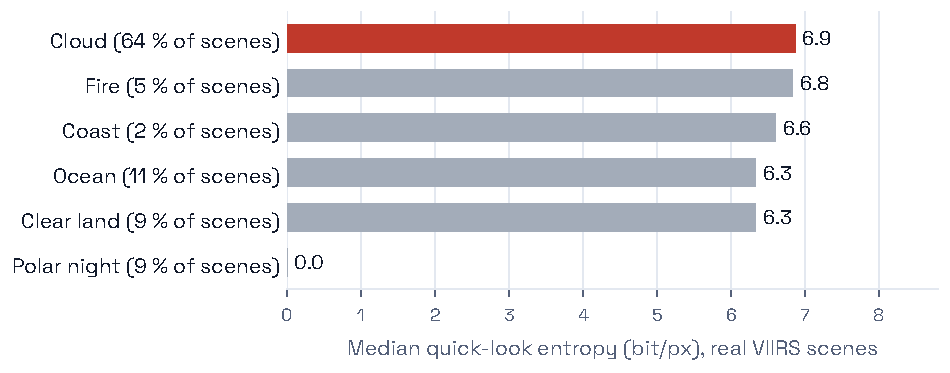
\includegraphics[width=0.78\textwidth]{fig_entropy}
\caption{Median quick-look entropy by real scene class. Clouds are the most textured scenes and the most common.}
\label{fig:entropy}
\end{figure}

\begin{figure}[H]
\centering
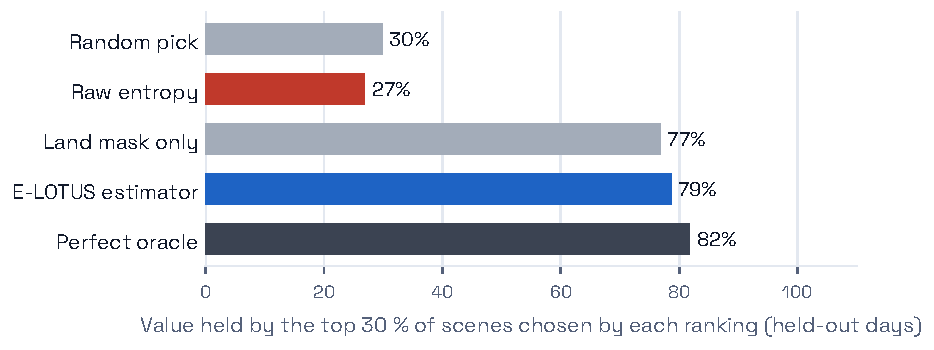
\includegraphics[width=0.78\textwidth]{fig_triage}
\caption{Value captured by the top 30\,\% of scenes on held-out days. Raw entropy is worse than random; the E-LOTUS estimator is within 3 points of an oracle.}
\label{fig:triage}
\end{figure}

% ====================================================================================
\section{Spacecraft and Resource Model}
Every controller, including the baselines, sees exactly the same orbit, images and hardware limits.
Only the decision rule changes.

\begin{table}[H]
\centering
\caption{Simulated spacecraft (all parameters in \texttt{kaio/config.py}).}
\small
\begin{tabularx}{\textwidth}{@{}l X@{}}
\toprule
\textbf{Subsystem} & \textbf{Model and main parameters} \\
\midrule
Power & 100\,Wh battery integrated with RK4, 0.95 charge/discharge efficiency, CV taper above 90\,\%; body-mounted panels (20\,W per face); 6.5\,W bus; payload load-shed below 20\,Wh. \\
Thermal & Lumped node, radiator to deep space ($\varepsilon=0.85$, $A=0.045$\,m$^2$), solar and Earth-IR loads; limit 45\,\textdegree C, hardware throttle 60\,\textdegree C. \\
Compute & Edge-AI module, 15\,W active (Jetson-Orin class); processing reduces an image to 3\,\% of its size and keeps 90\,\% of its information. \\
Links, storage & 10\,Mbps downlink, 100\,Mbps laser link to a sunlit neighbour, 8\,GB storage. \\
Workload & Poisson acquisitions (1 per 45\,s in sunlight, 1 per 120\,s in eclipse), $\approx$50\,MB per image; deadline 1.5\,h for fire alerts, 12\,h otherwise. \\
\bottomrule
\end{tabularx}
\end{table}

The thermal node follows
\begin{equation}
  C\,\frac{dT}{dt} = P_{\text{gpu}} + Q_{\text{sun}} + Q_{\text{IR}} - \varepsilon\,\sigma\,A\,T^4 ,
\end{equation}
and the battery energy $E$ is integrated with RK4 from solar input, bus load and payload load.

% ====================================================================================
\section{End-to-End Architecture}
\begin{figure}[H]
\centering
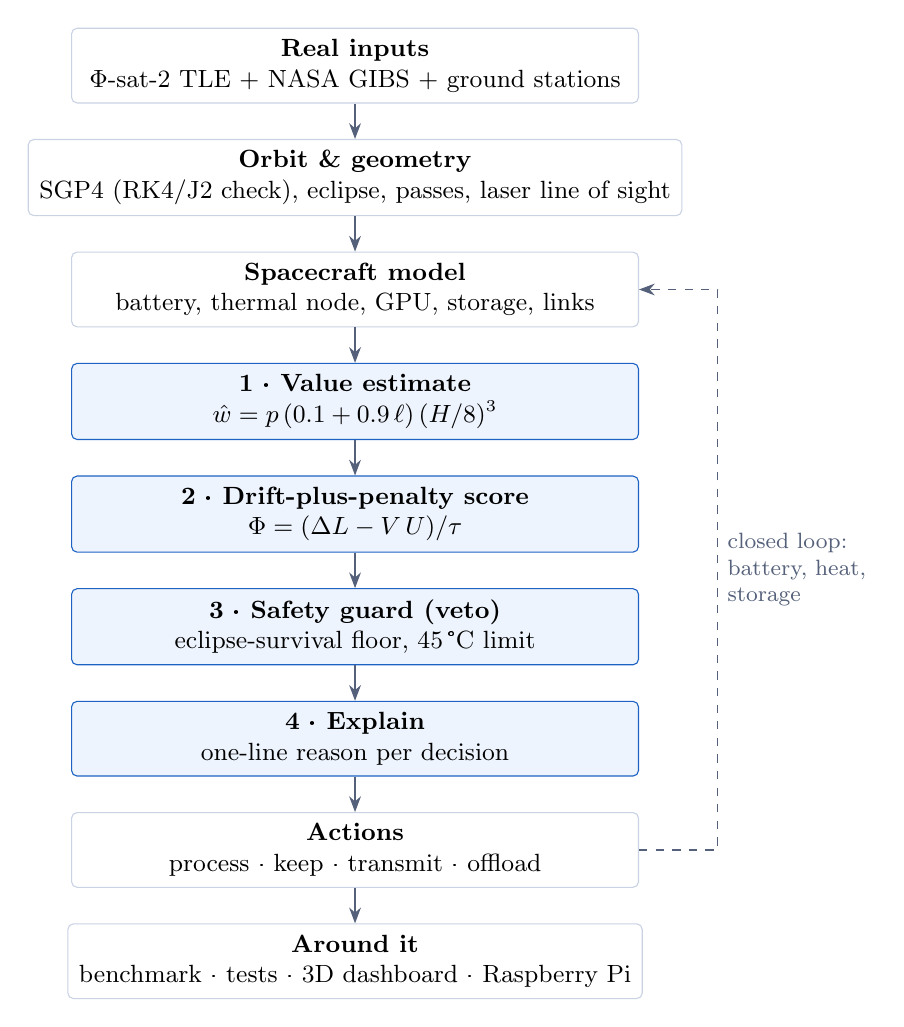
\begin{tikzpicture}[
  node distance=4.5mm,
  blk/.style={draw=kline,rounded corners=2pt,fill=white,align=center,minimum width=7.2cm,inner sep=4pt,font=\small},
  hot/.style={blk,draw=kblue,fill=kbluebg},
  arr/.style={-{Stealth[length=2mm]},color=kmuted}]
\node[blk] (a) {\textbf{Real inputs}\\ $\Phi$-sat-2 TLE + NASA GIBS + ground stations};
\node[blk,below=of a] (b) {\textbf{Orbit \& geometry}\\ SGP4 (RK4/J2 check), eclipse, passes, laser line of sight};
\node[blk,below=of b] (c) {\textbf{Spacecraft model}\\ battery, thermal node, GPU, storage, links};
\node[hot,below=of c] (d) {\textbf{1 \textperiodcentered{} Value estimate}\\ $\hat w = p\,(0.1+0.9\,\ell)\,(H/8)^3$};
\node[hot,below=of d] (e) {\textbf{2 \textperiodcentered{} Drift-plus-penalty score}\\ $\Phi=(\Delta L - V\,U)/\tau$};
\node[hot,below=of e] (f) {\textbf{3 \textperiodcentered{} Safety guard (veto)}\\ eclipse-survival floor, 45\,\textdegree C limit};
\node[hot,below=of f] (g) {\textbf{4 \textperiodcentered{} Explain}\\ one-line reason per decision};
\node[blk,below=of g] (h) {\textbf{Actions}\\ process \textperiodcentered{} keep \textperiodcentered{} transmit \textperiodcentered{} offload};
\node[blk,below=of h] (i) {\textbf{Around it}\\ benchmark \textperiodcentered{} tests \textperiodcentered{} 3D dashboard \textperiodcentered{} Raspberry Pi};
\foreach \x/\y in {a/b,b/c,c/d,d/e,e/f,f/g,g/h,h/i} \draw[arr] (\x) -- (\y);
\draw[arr,dashed] (h.east) -- ++(1.0,0) |- (c.east) node[pos=0.25,right,font=\footnotesize,color=kmuted,align=left]{closed loop:\\battery, heat,\\storage};
\end{tikzpicture}
\caption{End-to-end KAIO pipeline. The blue blocks are the E-LOTUS flight logic, run every 10\,s.}
\label{fig:flow}
\end{figure}

\begin{figure}[H]
\centering
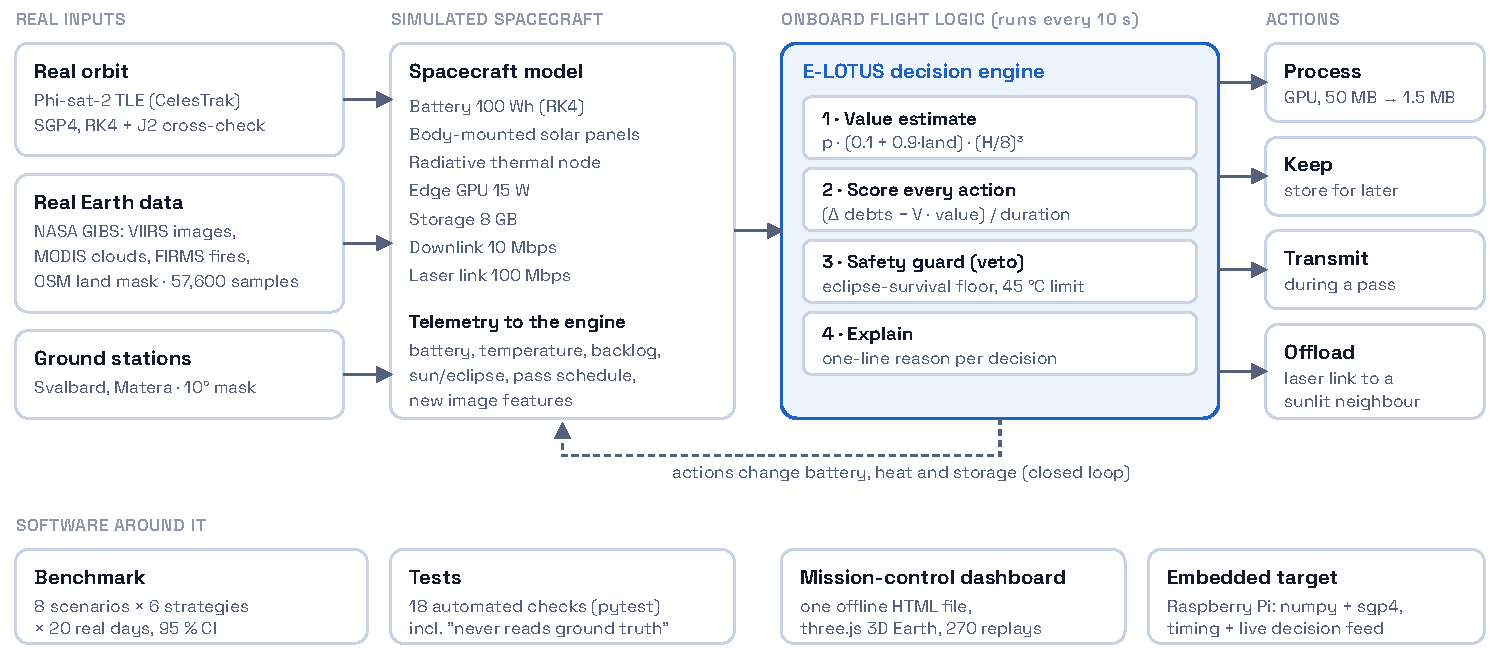
\includegraphics[width=\textwidth]{architecture}
\caption{Detailed architecture. Real inputs drive a simulated spacecraft; the E-LOTUS flight logic reads its telemetry and commands one of four actions. The surrounding software benchmarks, tests, visualises and runs the same code on embedded hardware.}
\label{fig:arch}
\end{figure}

The design separates three concerns, as in flight software: \textbf{the world} (orbit, data and
physics, all policy-independent), \textbf{the optimiser} (the E-LOTUS score) and \textbf{the protection}
(an independent safety guard).

% ====================================================================================
\section{The E-LOTUS Decision Engine}
\subsection{Value estimate (onboard)}
For each image the engine uses two numbers available onboard: the Shannon entropy $H$ of a quick-look
thumbnail and the land fraction $\ell$ of the footprint, read from a static land/water mask indexed by
the onboard position. The priority $p$ is 4 for a fire alert and 1 otherwise.
\begin{equation}
  \hat w = p\,(0.1 + 0.9\,\ell)\left(\frac{H}{8}\right)^{3} \quad\text{(optical)},\qquad
  \hat w = p\,(0.1 + 0.9\,\ell) \quad\text{(thermal-IR night)}.
\end{equation}

\subsection{Scoring: drift-plus-penalty}
The engine keeps three normalised ``debts'' small: the storage backlog $q/Q$, the energy debt $D_E$
below an eclipse-aware battery floor $E_{\min}(t)$, and the heat debt $D_T$ above $T_{\text{safe}}=45$\,\textdegree C:
\begin{equation}
  L = \tfrac12\left[\left(\frac{q}{Q}\right)^{2} + \left(\frac{D_E}{5\,\text{Wh}}\right)^{2} + \left(\frac{D_T}{5\,\text{K}}\right)^{2}\right],
\end{equation}
\begin{equation}
  \Phi_i(a) = \frac{\Delta L_i(a) - V\,U_i(a)}{\tau_i(a)}, \qquad a\in\{\text{process},\ \text{transmit},\ \text{offload}\}.
\end{equation}
For each stored image $i$ and action $a$, the engine predicts the change $\Delta L$ relative to keeping the
image, over the action duration $\tau$, with a linear energy budget and a first-order thermal model.
$U$ is the delivered value: $\hat w \times$ retained information $\times$ a freshness term that decays until the
deadline, minus an energy price that is zero when the solar array would otherwise be shunted. Free
resources are filled greedily with the most negative $\Phi$. $V=0.3$ is the single trade-off knob.

This is the drift-plus-penalty rule of Lyapunov optimisation~\cite{neely}. We use it as a principled scoring
rule; its textbook bound assumes stationary arrivals, which an orbit does not provide, so every claim in
this report is empirical.

\subsection{Safety guard}
An independent layer checks each proposed job before it starts, like FDIR in flight software. It blocks
the job if, at its end:
\begin{itemize}
  \item the battery would fall below the energy needed to carry the platform through the current or next eclipse plus a reserve:
  \begin{equation} E(t+\tau) \;\ge\; E_{\min}(t) = P_{\text{bus}}\; t_{\text{eclipse}}(t) + E_{\text{reserve}} ; \end{equation}
  \item the computer would exceed 45\,\textdegree C (fire alerts may use the margin up to the 60\,\textdegree C hardware limit).
\end{itemize}
Blocked jobs are logged with their reason.

\subsection{Storage eviction and explanations}
When storage is full, the engine deletes the items with the lowest expected value per megabyte first (the
rule-based baselines get the same rule, for fairness). Every started job carries a one-line reason built
only from onboard quantities, for example:

\begin{keybox}
\small\ttfamily Process now: est. value 0.68 (optical H 7.5, land 79\,\%). 20\,MB raw $\rightarrow$ 0.6\,MB product,
next pass in 476\,min; battery 69\,Wh after (floor 20), 9.3\,\textdegree C.
\end{keybox}

\begin{keybox}
\textbf{Onboard information set.} At decision time $t$ the engine may use battery and temperature
housekeeping, the uplinked pass schedule, eclipse times from the onboard propagator, the land/water mask,
the thumbnail entropy and the alert flag. It cannot use the cloud fraction, the hidden value, or any
information after $t$.
\end{keybox}

% ====================================================================================
\section{Evaluation Protocol}
\begin{itemize}
  \item \textbf{Days:} 20 real days, each an independent 24\,h run from 00:00 UTC on 2026-08-26\,+\,$d$; workload seed $2026+d$; every strategy sees the same images on a given day.
  \item \textbf{Strategies:} Always-Transmit (bent pipe); Greedy-Process (process everything); Store-and-Forward (no onboard compute); Rule-Based (hand-tuned rule engine with the same value estimate and battery/temperature thresholds); Bandwidth-Rules (Rule-Based plus pass-capacity awareness).
  \item \textbf{Scenarios:} nominal plus seven single-resource degradations, fixed in advance and applied without retuning any controller.
  \item \textbf{Statistics:} mean $\pm$ 95\,\% confidence interval (Student $t$ over days) and the number of days on which E-LOTUS beats each baseline.
  \item \textbf{Tuning hygiene:} $V$ and the debt weights were selected on a different workload seed.
\end{itemize}
\strip{\textbf{8} scenarios \;$|$\; \textbf{6} strategies \;$|$\; \textbf{20} real days \;$|$\; \textbf{1,360} runs incl.\ ablations \;$|$\; 95\,\% CI}

% ====================================================================================
\section{Results}
\subsection{Quality of decisions}
\begin{figure}[H]
\centering
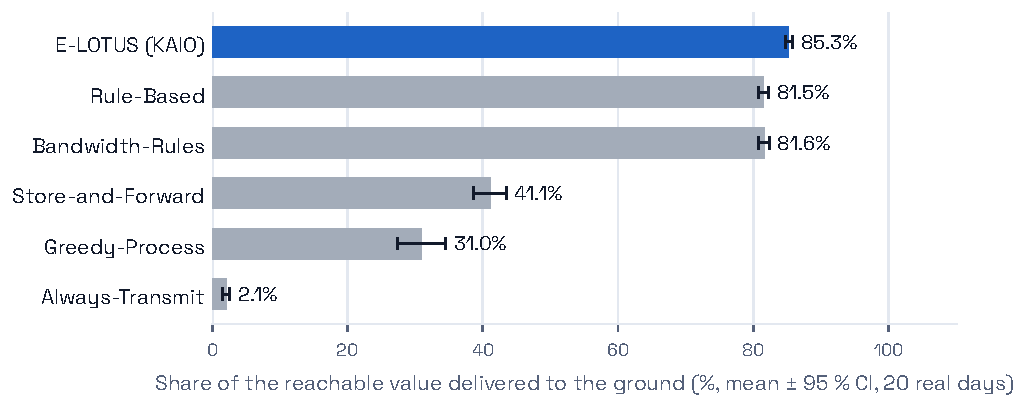
\includegraphics[width=0.85\textwidth]{fig_value}
\caption{Value delivered, nominal scenario. E-LOTUS 85.3\,$\pm$\,0.6\,\%, Rule-Based 81.5\,$\pm$\,0.7\,\%, Bandwidth-Rules 81.6\,$\pm$\,0.8\,\%. The intervals do not overlap.}
\label{fig:value}
\end{figure}

\subsection{All performance indicators}
\begin{table}[H]
\centering
\caption{Nominal scenario, mean of 20 real days.}
\small
\begin{tabular}{@{}llrrrrr@{}}
\toprule
\textbf{Indicator} & \textbf{Metric} & \textbf{E-LOTUS} & \textbf{Rules} & \textbf{Greedy} & \textbf{S\&F} & \textbf{Tx} \\
\midrule
Quality & Value delivered (\%) & \textbf{85.3} & 81.5 & 31.0 & 41.1 & 2.1 \\
        & Fire alerts in time (\%) & 72.7 & 72.8 & 21.4 & 63.7 & 0.0 \\
Completed tasks & Delivered or triaged (\%) & \textbf{71.9} & 47.8 & 47.2 & 7.5 & 7.4 \\
Energy & Payload energy (Wh/day) & 193 & 159 & 264 & 52 & 52 \\
       & Lowest battery (\%) & 69 & 68 & 19 & 69 & 69 \\
Latency & Mean (min) & 120 & 134 & 239 & 73 & 160 \\
        & 95th percentile (min) & 442 & 473 & 477 & 163 & 233 \\
Utilisation & GPU duty cycle (\%) & 44 & 33 & 71 & 0 & 0 \\
            & Downlink use in passes (\%) & 85 & 100 & 28 & 100 & 100 \\
Safety & Time above 45\,\textdegree C (\%) & 0.1 & 0.0 & 53.4 & 0.0 & 0.0 \\
       & Payload load-shed (\%) & \textbf{0.0} & 0.0 & 18.5 & 0.0 & 0.0 \\
\bottomrule
\end{tabular}
\end{table}
{\footnotesize\color{kmuted} Rules = Rule-Based, S\&F = Store-and-Forward, Tx = Always-Transmit.}

\begin{itemize}
  \item \textbf{Quality:} the most value (+3.7 pts over the rule engine), and the same fire-alert performance as the best strategies.
  \item \textbf{Completed tasks:} 71.9\,\% against 47.8\,\%; laser offload in eclipse and value-aware eviction keep more images moving.
  \item \textbf{Energy:} E-LOTUS spends more payload energy (193 vs 159\,Wh/day), but it is solar power that would otherwise be shunted: the battery never drops below 69\,\% and there is no load-shed. Greedy-Process drains it to 19\,\% and sheds the payload 19\,\% of the time.
  \item \textbf{Latency:} lowest mean latency of the processing strategies (120 vs 134\,min).
  \item \textbf{Utilisation:} GPU 44\,\%, 85\,\% of pass capacity; time above 45\,\textdegree C is 0.1\,\% (fire alerts only).
\end{itemize}

\begin{resultbox}
\textbf{E-LOTUS beats a tuned rule engine with the same information}\\
85.3\,\% vs 81.5\,\% of the reachable value, better on 20/20 real days, with no load-shed.
\end{resultbox}

\subsection{One real day}
\begin{figure}[H]
\centering
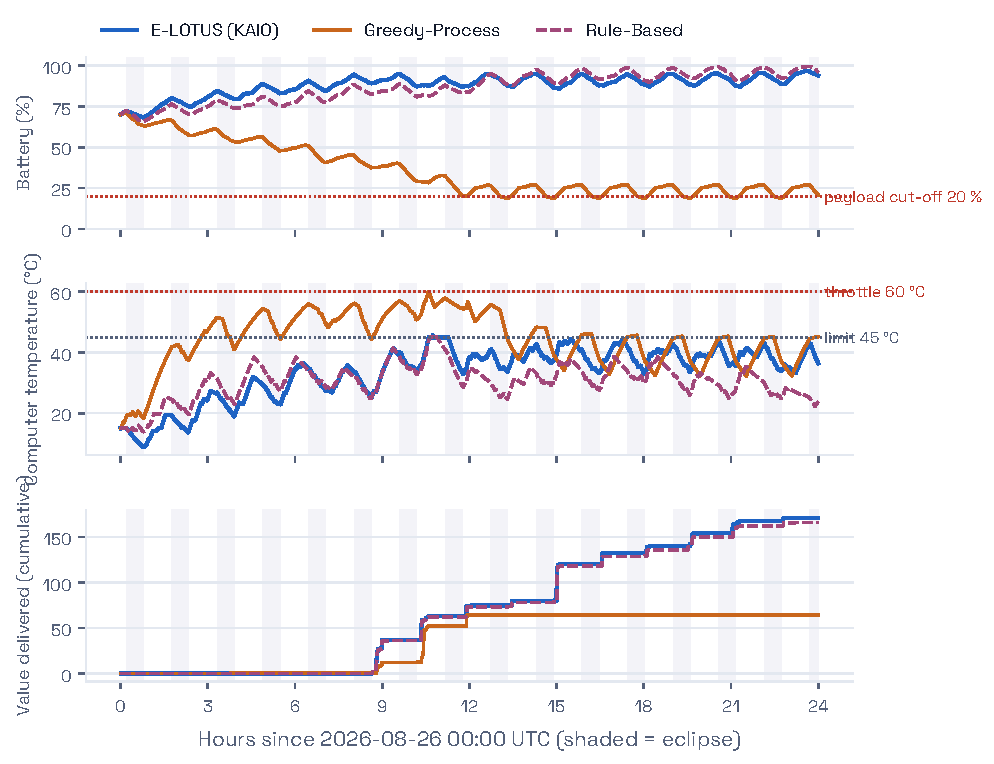
\includegraphics[width=0.85\textwidth]{fig_telemetry}
\caption{One real day (2026-08-26). Greedy processing drains the battery to the payload cut-off and runs hot; E-LOTUS keeps the battery high, the computer under 45\,\textdegree C, and delivers the most value.}
\label{fig:telemetry}
\end{figure}

% ====================================================================================
\section{Robustness and Ablations}
\begin{figure}[H]
\centering
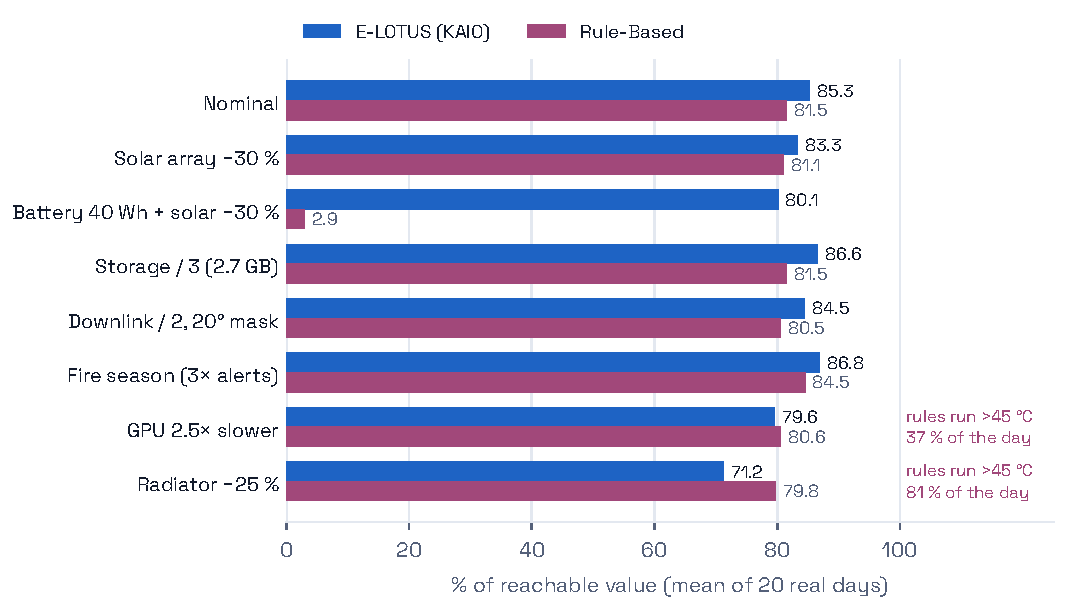
\includegraphics[width=0.85\textwidth]{fig_stress}
\caption{Eight scenarios, 20 real days each, no retuning.}
\label{fig:stress}
\end{figure}

\begin{table}[H]
\centering
\caption{Stress scenarios (\% of reachable value, mean $\pm$ 95\,\% CI).}
\small
\begin{tabular}{@{}lccccc@{}}
\toprule
\textbf{Scenario} & \textbf{E-LOTUS} & \textbf{Rule-Based} & \textbf{BW-Rules} & \textbf{Days won} & \textbf{Rules $>$45\,\textdegree C} \\
\midrule
Nominal & \textbf{85.3 $\pm$ 0.6} & 81.5 $\pm$ 0.7 & 81.6 $\pm$ 0.8 & 20/20 & 0\,\% \\
Solar array $-30$\,\% & \textbf{83.3 $\pm$ 0.5} & 81.1 $\pm$ 0.8 & 76.0 $\pm$ 1.8 & 20/20 & 0\,\% \\
Battery 40\,Wh + solar $-30$\,\% & \textbf{80.1 $\pm$ 0.7} & 2.9 $\pm$ 0.2 & 2.9 $\pm$ 0.2 & 20/20 & 0\,\% \\
Storage / 3 (2.7\,GB) & \textbf{86.6 $\pm$ 0.5} & 81.5 $\pm$ 0.7 & 81.6 $\pm$ 0.8 & 20/20 & 0\,\% \\
Downlink / 2, 20\textdegree{} mask & \textbf{84.5 $\pm$ 0.6} & 80.5 $\pm$ 0.8 & 80.3 $\pm$ 1.0 & 20/20 & 0\,\% \\
Fire season (3$\times$ alerts) & \textbf{86.8 $\pm$ 0.5} & 84.5 $\pm$ 0.7 & 83.9 $\pm$ 1.1 & 20/20 & 0\,\% \\
GPU 2.5$\times$ slower & 79.6 $\pm$ 0.8 & \textbf{80.6 $\pm$ 0.8} & 75.3 $\pm$ 1.8 & 2/20 & 37\,\% \\
Radiator $-25$\,\% & 71.2 $\pm$ 1.4 & \textbf{79.8 $\pm$ 0.9} & 76.9 $\pm$ 1.9 & 0/20 & 81\,\% \\
\bottomrule
\end{tabular}
\end{table}

\textbf{Wins (6/8).} With a 40\,Wh battery and weaker panels, the rule engine's fixed 50\,\% battery
threshold coincides with the shutdown floor and it collapses (2.9\,\%); E-LOTUS's eclipse-survival floor
is computed from the orbit and adapts automatically (80.1\,\%).

\textbf{Losses (2/8).} With a slower GPU or a weaker radiator the rule engine scores higher, but only by
running above 45\,\textdegree C for 37\,\% and 81\,\% of the day. If operators allow 60\,\textdegree C for every
job, E-LOTUS reaches 82.1\,\% in the radiator case. The thermal limit is an operator setting, not a limit of
the method.

\subsection{Ablations}
\begin{table}[H]
\centering
\caption{Contribution of each component (\% of reachable value).}
\small
\begin{tabular}{@{}lcccc@{}}
\toprule
\textbf{Variant} & \textbf{Nominal} & \textbf{Solar $-30$\,\%} & \textbf{Battery 40\,Wh} & \textbf{Radiator $-25$\,\%} \\
\midrule
Full E-LOTUS & 85.3 & 83.3 & 80.1 & 71.2 \\
Without entropy (land mask only) & 87.1 & 78.3 & 66.3 & 69.3 \\
Without land mask (raw entropy) & 83.5 & 51.7 & 41.7 & 63.4 \\
Without laser offload & 83.7 & 81.6 & 77.8 & 67.0 \\
Without eclipse-aware floor & 85.3 & 82.9 & 79.2 & 71.2 \\
\bottomrule
\end{tabular}
\end{table}
\begin{itemize}
  \item The land-mask prior is the key ingredient: raw entropy alone loses 2 to 38 points.
  \item Entropy pays off when resources are scarce (+2 to +14 points).
  \item Laser offload adds 1.6 to 4.2 points; the eclipse-aware floor matters under energy stress.
\end{itemize}

% ====================================================================================
\section{Validation and Reproducibility}
Before any result is reported, the pipeline verifies, with 18 automated \texttt{pytest} checks:
\begin{itemize}
  \item SGP4 and the RK4 + $J_2$ integrator agree within 25\,km over 6\,h;
  \item battery, temperature and storage stay within physical bounds;
  \item quick-look entropy lies in $[0, 8]$ bit/px;
  \item the safety guard vetoes jobs that would break the eclipse floor or the thermal limit;
  \item runs are deterministic for a given seed;
  \item the engine never reads the hidden ground-truth value;
  \item every image is accounted for exactly once (delivered, stored, triaged or evicted).
\end{itemize}

\begin{table}[H]
\centering
\caption{Representative verification checks.}
\small
\begin{tabular}{@{}lc@{}}
\toprule
\textbf{Check} & \textbf{Result} \\
\midrule
SGP4 vs RK4/$J_2$ cross-check & \pass \\
Physics bounds (battery, temperature, storage) & \pass \\
Entropy limits & \pass \\
Safety-guard vetoes & \pass \\
Deterministic replay & \pass \\
Engine never reads ground truth (shuffle test) & \pass \\
Image bookkeeping & \pass \\
Safety properties (no load-shed, eclipse survival) & \pass \\
\bottomrule
\end{tabular}
\end{table}

\begin{resultbox}
\textbf{18 / 18 automated checks passed.} Every figure and table is regenerated from \texttt{results/summary.json} by scripts.
\end{resultbox}

% ====================================================================================
\section{Feasibility and Embedded Implementation}
Every input the engine uses exists on a real satellite: battery and temperature housekeeping, a pass
schedule computed on the ground and uplinked, eclipse times from the onboard propagator, a static
land/water mask indexed by GNSS position, and a thumbnail entropy. The engine needs no GPU and no
training; its only dependencies are \texttt{numpy} and \texttt{sgp4}. ESA's $\Phi$-sat-1 already discarded
cloudy images onboard~\cite{phisat}; KAIO flies the real orbit of its successor.

\begin{table}[H]
\centering
\caption{Embedded timing, measured on the \benchboard.}
\small
\begin{tabular}{@{}lr@{}}
\toprule
\textbf{Quantity} & \textbf{Value} \\
\midrule
Decision time (median / p99 / worst) & \decmedian{} / \decpninetynine{} / \decmax{}\,ms \\
Decision cycle required & every 10\,s \\
CPU used by the engine over a full real day & \cpuduty\,\% of one core \\
Quick-look entropy, one $32\times32$ thumbnail & \entropyus\,$\mu$s \\
Peak memory, whole program & \peakram\,MB \\
\bottomrule
\end{tabular}
\end{table}
{\footnotesize\color{kmuted} Regenerate with \texttt{python3 onboard/pi\_benchmark.py} on the target board.}

% ====================================================================================
\section{Software Platform}
\subsection{Flight logic and simulation --- Python}
Package \texttt{kaio/}: \texttt{orbit}, \texttt{workload}, \texttt{estimator}, \texttt{physics},
\texttt{safety}, \texttt{engine}, \texttt{baselines}, \texttt{simulator}, \texttt{scenarios}. Every
assumption lives in \texttt{config.py}. Dependencies: \texttt{numpy}, \texttt{sgp4}, \texttt{scipy}.

\subsection{Benchmark}
\texttt{benchmark.py} runs 8 scenarios $\times$ 6 strategies $\times$ 20 days plus ablations (1,360 runs) in
parallel and writes \texttt{summary.json}, \texttt{summary.md} and a per-run CSV.

\subsection{Mission-control dashboard}
One self-contained offline HTML file (HTML, CSS, JavaScript, three.js): a 3D Earth with the real orbit,
an orbit designer (80 what-if orbits), a 24\,h replay of 270 what-if missions, the benchmark, the real-data
findings, and light/dark modes. It needs no server and no internet.

\begin{figure}[H]
\centering
\begin{minipage}{0.49\textwidth}\centering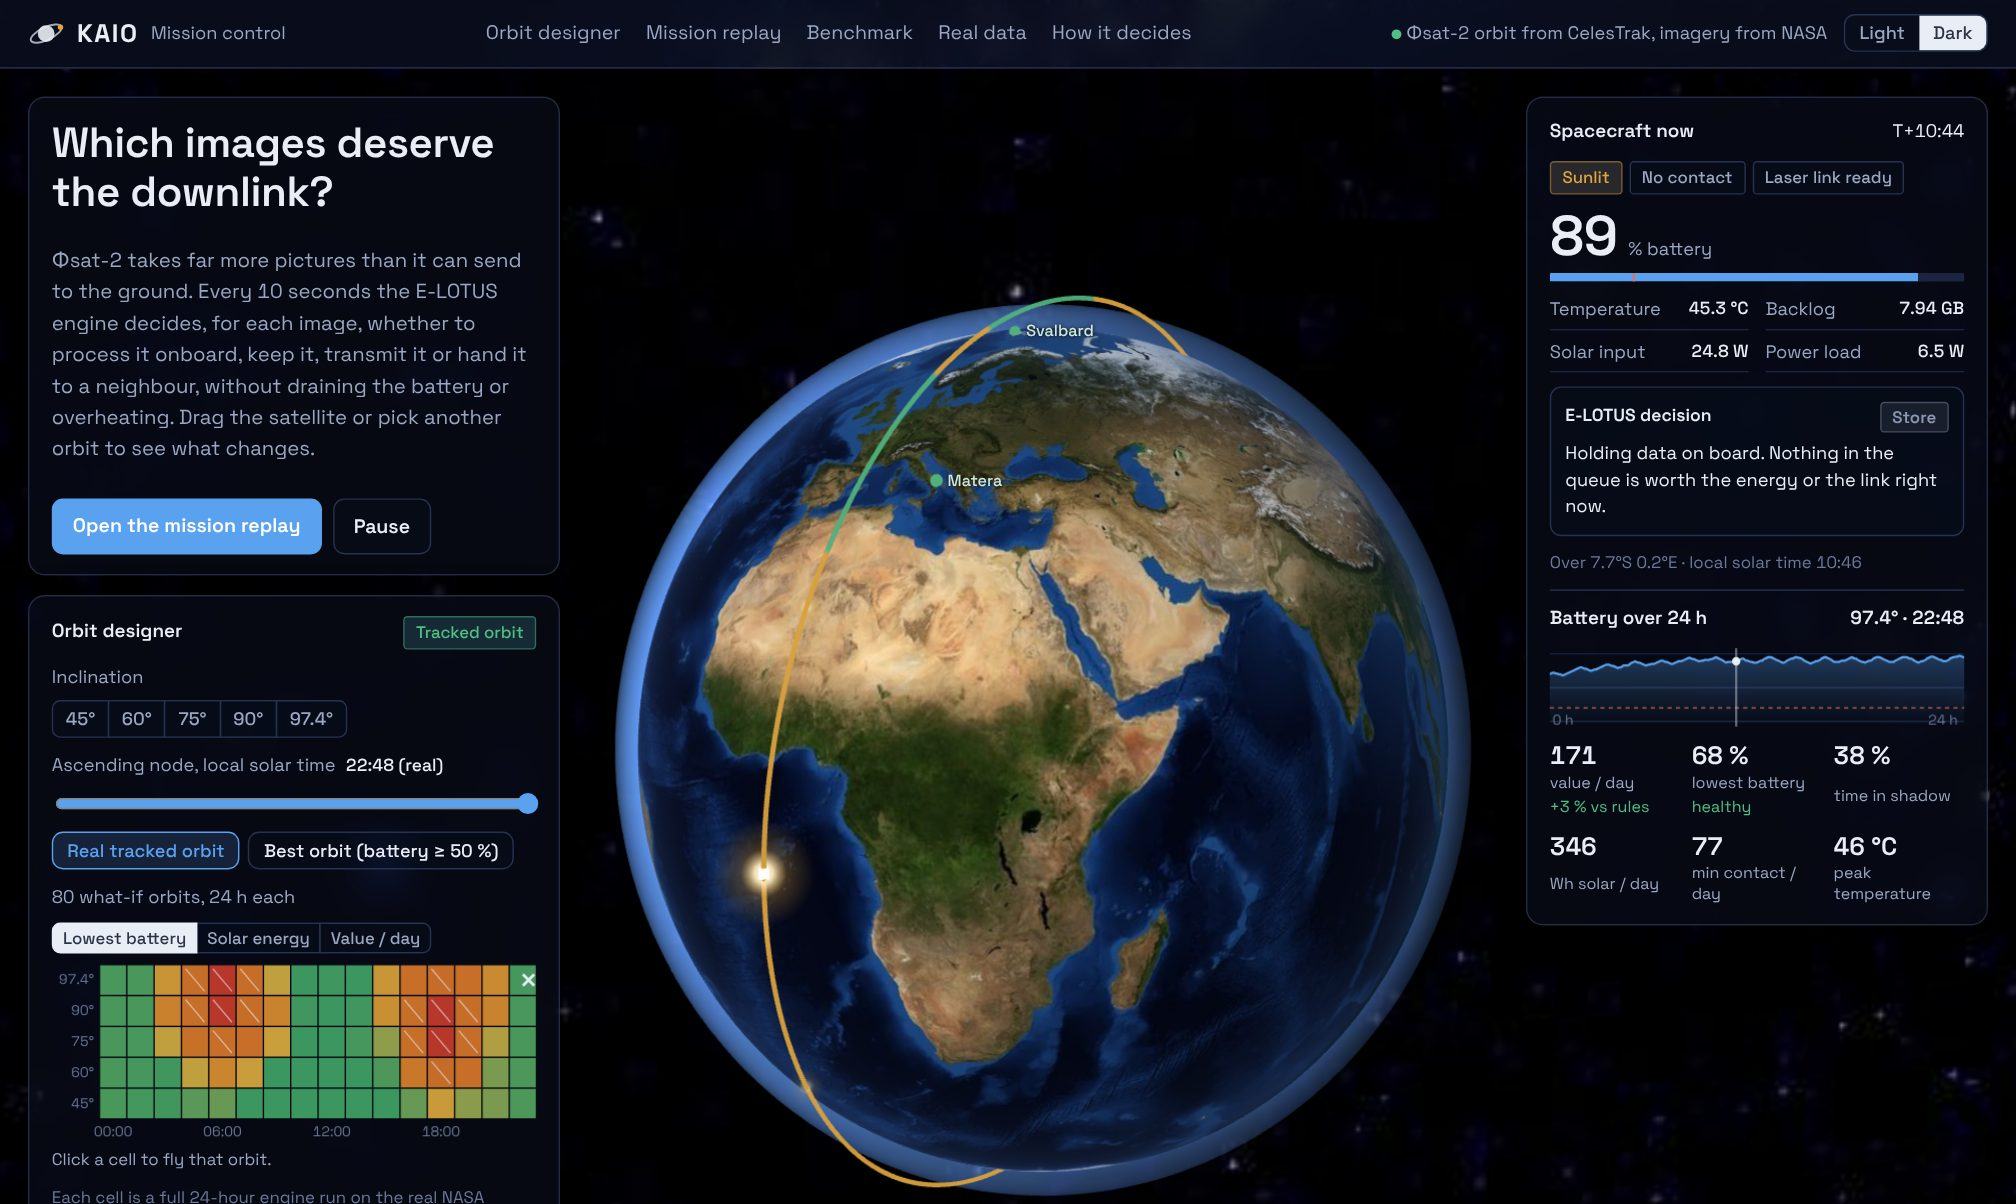
\includegraphics[width=\textwidth]{dash_hero_dark}\end{minipage}\hfill
\begin{minipage}{0.49\textwidth}\centering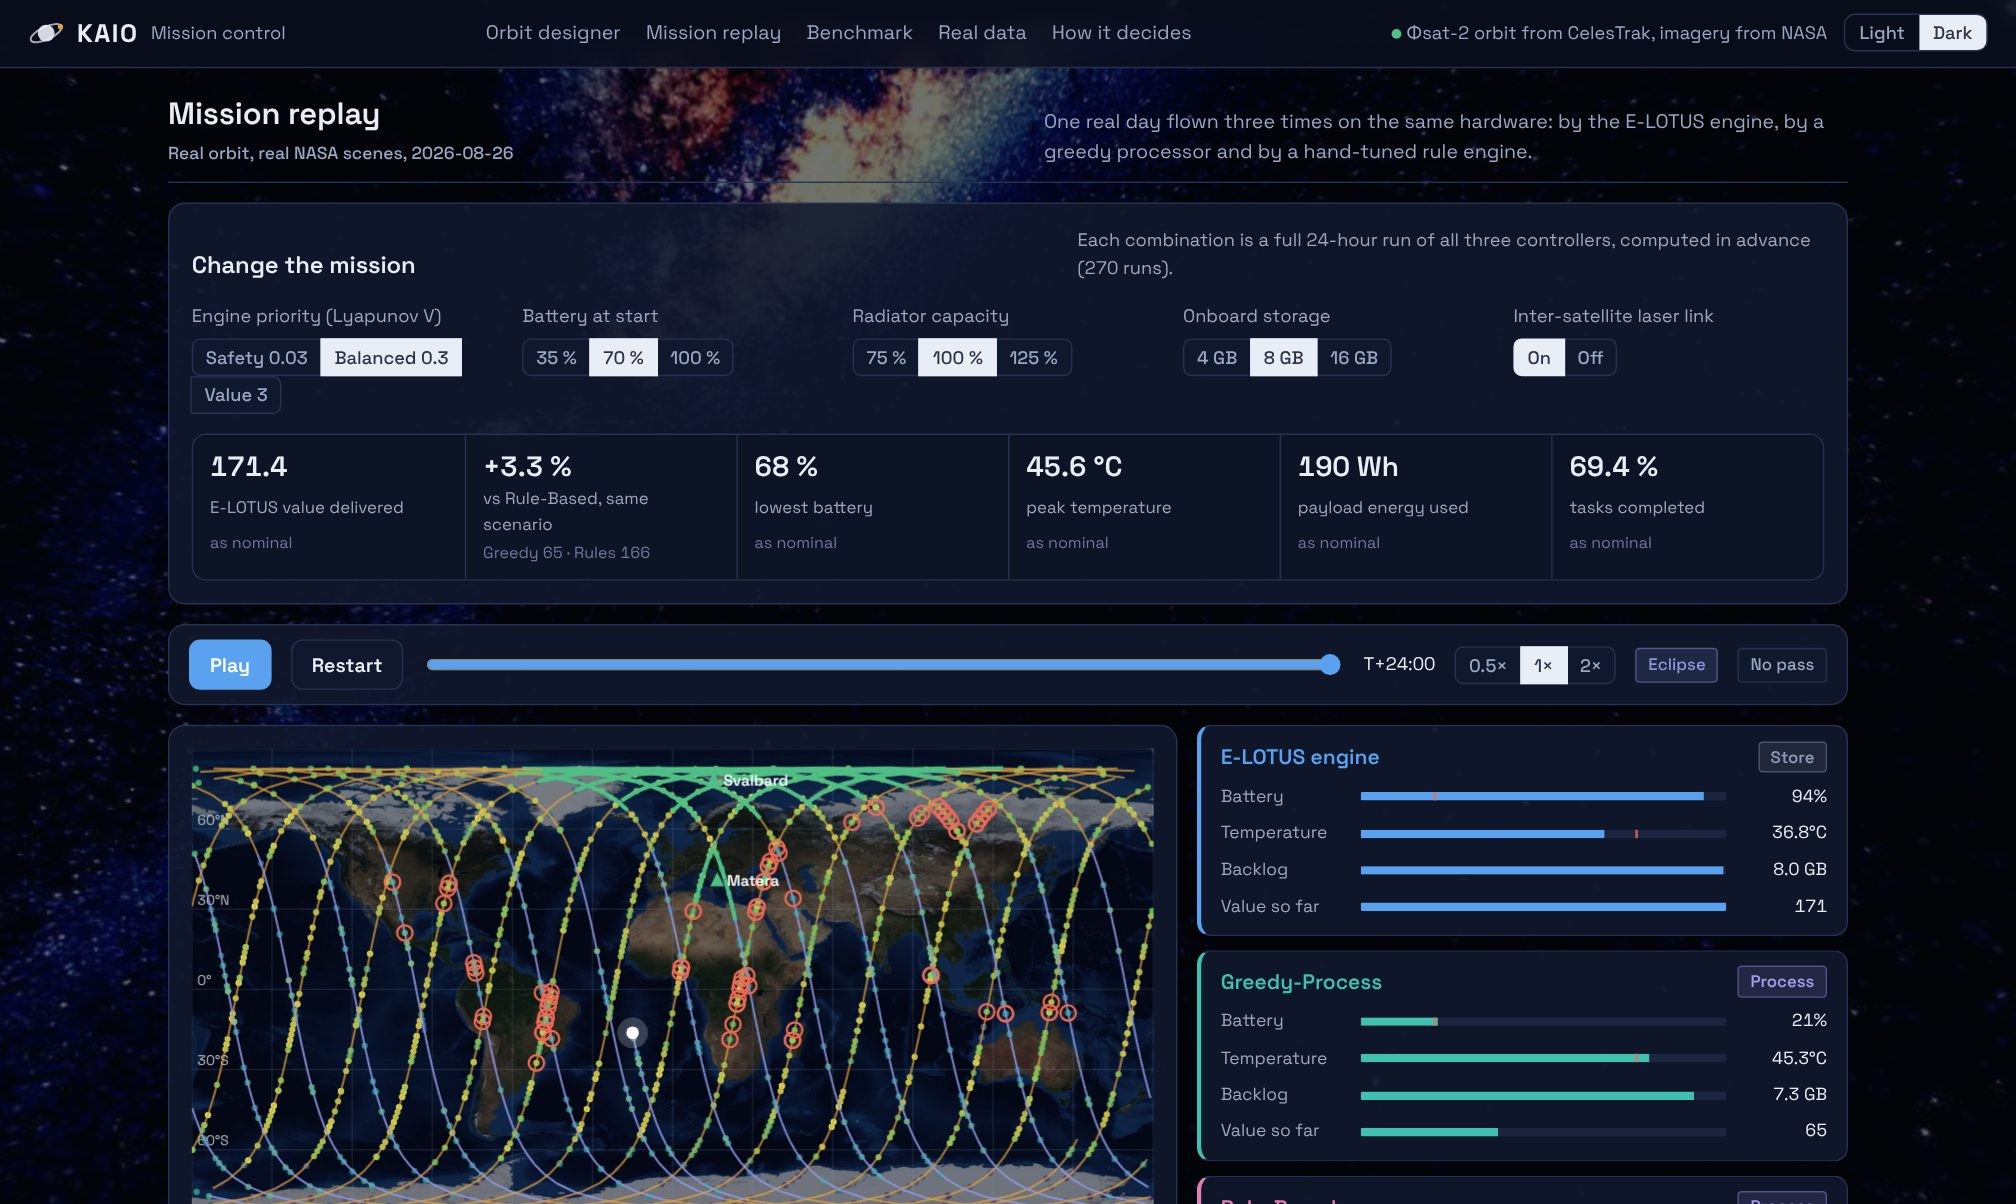
\includegraphics[width=\textwidth]{dash_replay_dark}\end{minipage}
\caption{Dashboard: (left) 3D Earth flying the real $\Phi$-sat-2 orbit; (right) one real day replayed by E-LOTUS, a greedy processor and a rule engine.}
\label{fig:dash1}
\end{figure}

\begin{figure}[H]
\centering
\begin{minipage}{0.49\textwidth}\centering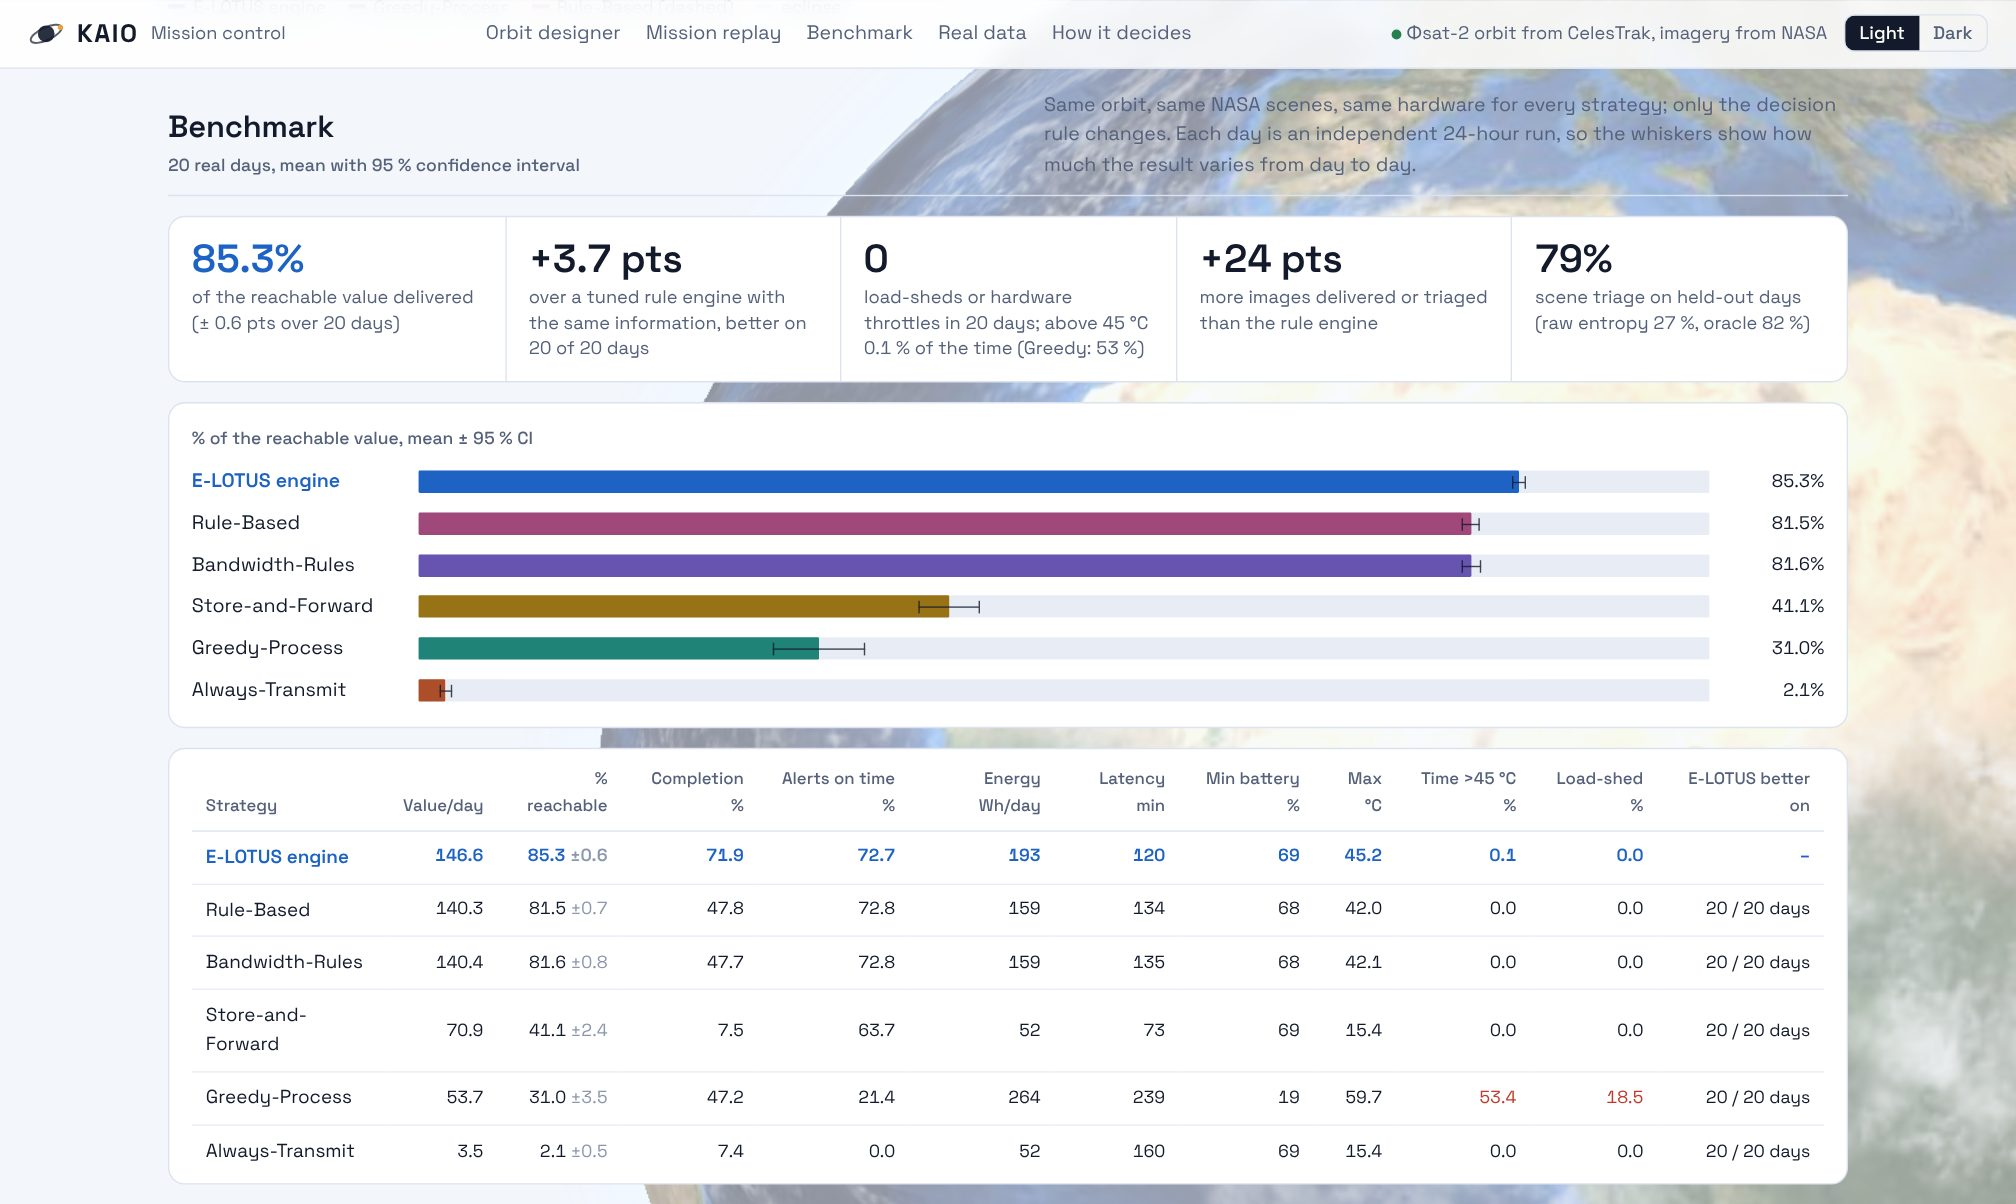
\includegraphics[width=\textwidth]{dash_bench_light}\end{minipage}\hfill
\begin{minipage}{0.49\textwidth}\centering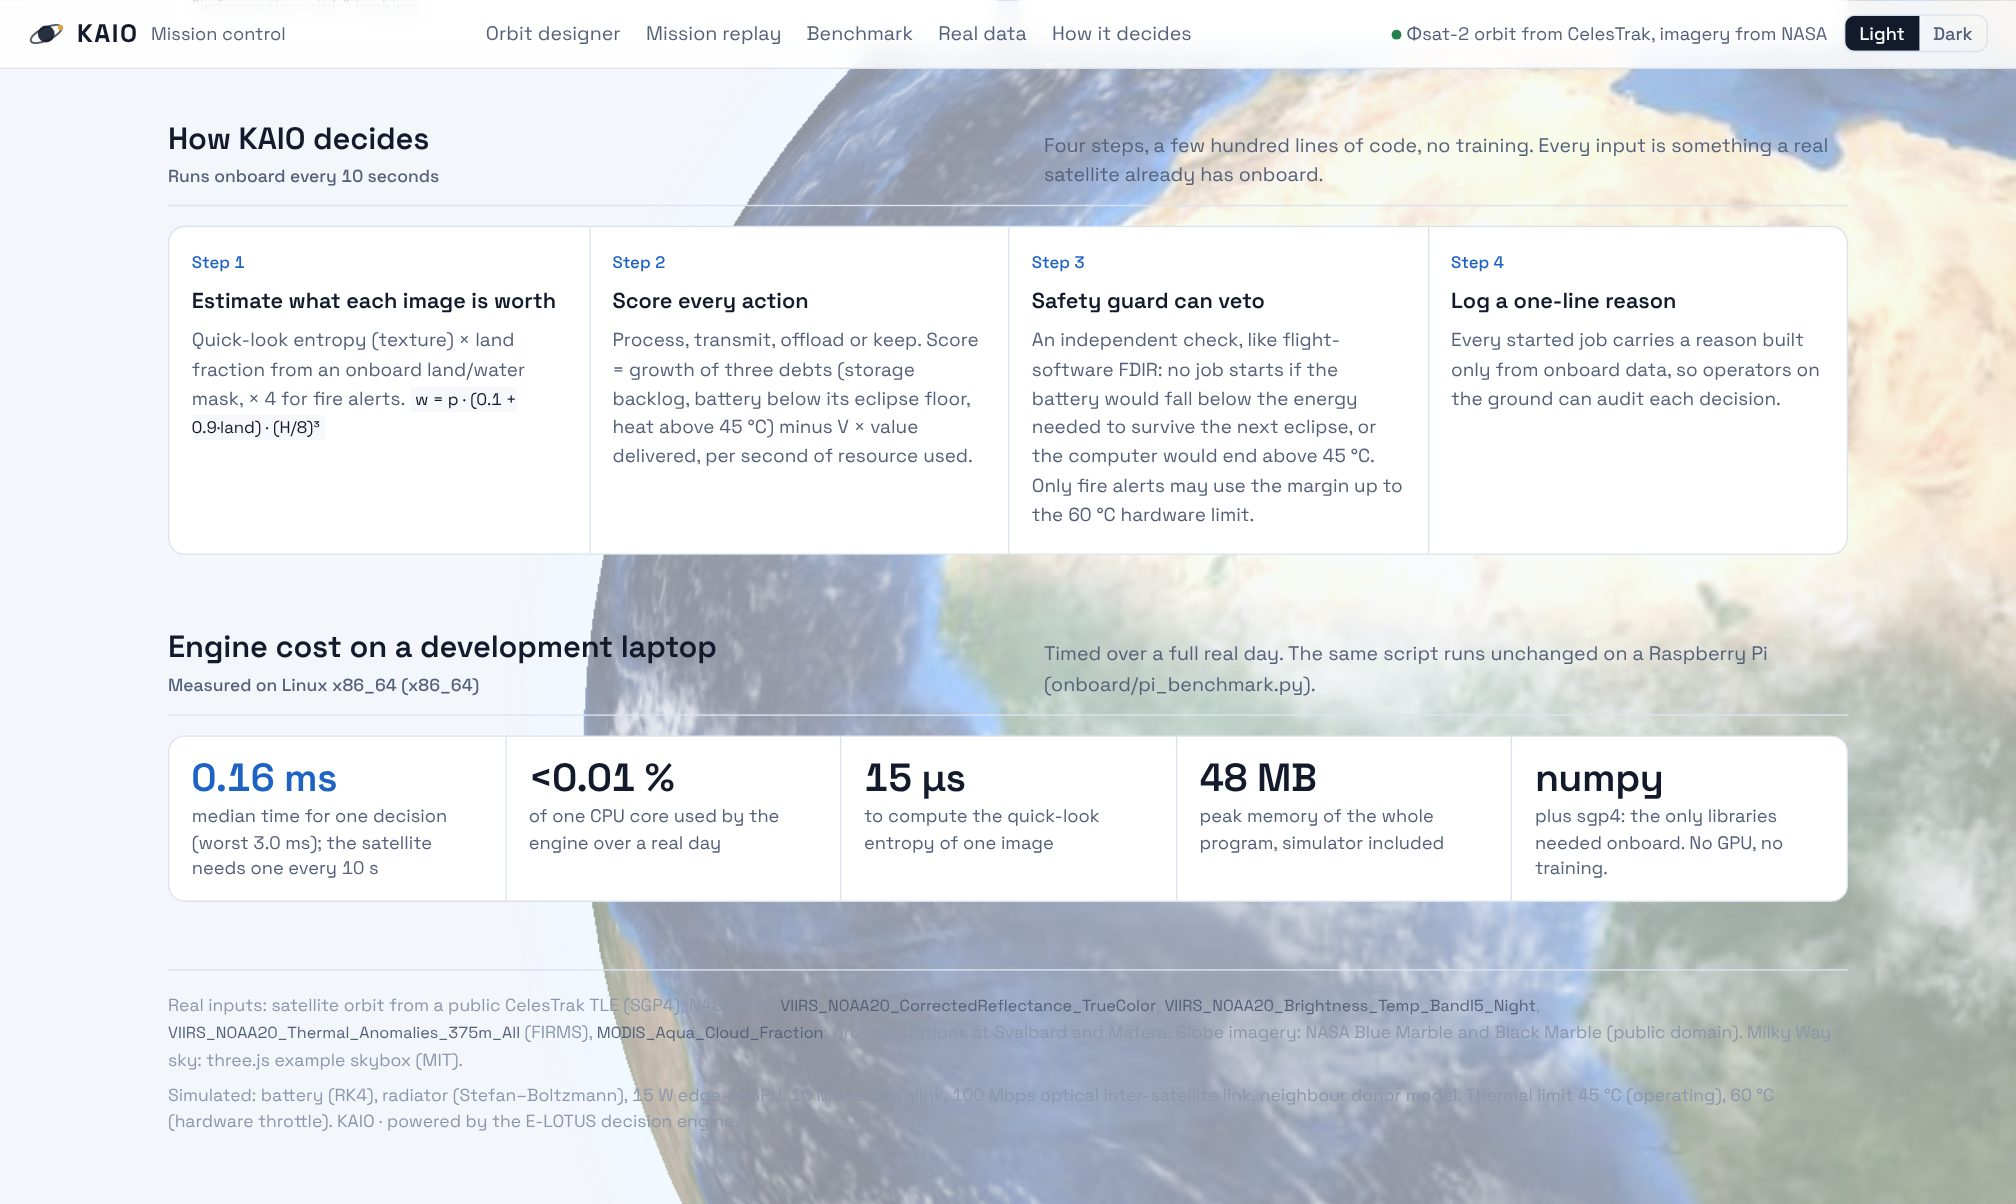
\includegraphics[width=\textwidth]{dash_how_light}\end{minipage}
\caption{Dashboard in light mode: (left) benchmark results; (right) how the engine decides.}
\label{fig:dash2}
\end{figure}

\subsection{Embedded target --- Raspberry Pi}
\texttt{onboard/pi\_benchmark.py} measures timing, CPU and memory; \texttt{onboard/live\_demo.py} prints a
live decision feed with the reason for each decision.

% ====================================================================================
\section{Engineering Defensibility}
The project is built around five principles.
\begin{enumerate}
  \item \textbf{No ground-truth leakage.} The engine never reads the hidden value; a shuffle test proves it.
  \item \textbf{Same world for every strategy.} Orbit, images and hardware limits are identical; only the decision rule changes.
  \item \textbf{Safety is separate from optimisation.} An independent guard can veto any job, like FDIR.
  \item \textbf{No retuning under stress.} Scenarios were fixed in advance; losses are reported.
  \item \textbf{Simulation is separated from measurement.} Real data drive the world; the spacecraft hardware is a model and is labelled as such.
\end{enumerate}

\begin{keybox}
\textbf{Reproducibility principle.} Every number in this report is produced by scripts from the
repository (\texttt{\repourl}); nothing is copied by hand.
\end{keybox}

% ====================================================================================
\section{Limitations}
\begin{enumerate}
  \item The spacecraft hardware and the ground-truth value model are assumptions, not a specific mission; operators would calibrate scene value.
  \item Pass and eclipse forecasts come from the same propagated orbit and are therefore exact.
  \item The laser-link neighbour is modelled; without it, E-LOTUS still beats the rule engines.
  \item The TLE epoch is 26 Sep 2026, so August positions are propagated about one month backwards (kilometre-level error, small against 313\,km footprints).
  \item The imagery days are shared between tuning and evaluation; only the acquisition streams differ.
  \item Baselines are heuristics; a hindsight-optimal schedule is future work.
\end{enumerate}

% ====================================================================================
\section{Conclusion and Future Work}
KAIO shows that a satellite can decide onboard, every 10\,s and in under a millisecond, which images
deserve the downlink, using only information it really has. The validated system demonstrates:
\begin{itemize}
  \item the real orbit of $\Phi$-sat-2 and 57,600 real NASA footprints;
  \item 85.3\,\% of the reachable value, +3.7 points over a tuned rule engine, 20/20 days won;
  \item 71.9\,\% of tasks completed against 47.8\,\%;
  \item no payload load-shed, battery never below 69\,\%, 0.1\,\% of the time above 45\,\textdegree C;
  \item 6/8 stress scenarios won without retuning, the two losses explained;
  \item 18/18 automated checks and a fully scripted benchmark;
  \item an offline 3D dashboard and an embedded Raspberry Pi implementation.
\end{itemize}

\begin{resultbox}
\large Decide onboard, using only what the satellite really knows.
\end{resultbox}

\subsection*{Methodology and roadmap}
We built two independent prototypes, reviewed them against each other and merged them into KAIO: the
real-data world, the E-LOTUS engine and the dashboard from one; the tested package structure,
explanations, bandwidth-aware baseline and statistical protocol from the other. The review found that the
earlier engine spent 10\,\% of the time above 45\,\textdegree C; the safety guard reduced this to 0.1\,\%.

\begin{table}[H]
\centering
\caption{Roadmap to flight.}
\small
\begin{tabularx}{\textwidth}{@{}l X X@{}}
\toprule
\textbf{When} & \textbf{Milestone} & \textbf{Success criterion} \\
\midrule
Done & Engine, safety guard, real-data simulation, benchmark, dashboard, embedded run & All results reproducible from scripts \\
+3 months & Hardware-in-the-loop on a flight-like computer; imperfect pass and eclipse forecasts; sensor noise & Same ranking with realistic forecast errors \\
+6 months & Small onboard cloud-screening network replacing the static land prior; hindsight-optimal comparison & Triage within 3 points of the oracle; optimality gap quantified \\
+12 months & Constellation coordination; CubeSat flight-experiment partnership & Flight-software integration plan and test campaign \\
\bottomrule
\end{tabularx}
\end{table}

% ====================================================================================
\begin{thebibliography}{9}
\bibitem{neely} M.~J. Neely, \emph{Stochastic Network Optimization with Application to Communication and Queueing Systems}, Morgan \& Claypool, 2010.
\bibitem{sgp4} D.~A. Vallado, P.~Crawford, R.~Hujsak, T.~S. Kelso, ``Revisiting Spacetrack Report \#3,'' AIAA/AAS Astrodynamics Specialist Conference, 2006.
\bibitem{gibs} NASA Global Imagery Browse Services (GIBS); NASA FIRMS active-fire data; CelesTrak element sets.
\bibitem{phisat} G.~Giuffrida \emph{et al.}, ``The $\Phi$-Sat-1 mission: the first on-board deep neural network demonstrator for satellite Earth observation,'' \emph{IEEE Trans.\ Geoscience and Remote Sensing}, 2022.
\bibitem{shannon} C.~E. Shannon, ``A Mathematical Theory of Communication,'' \emph{Bell System Technical Journal}, 1948.
\end{thebibliography}

\paragraph{AI-use statement.} We used Claude (Anthropic) as a coding and writing assistant: to review and
merge the two prototypes, implement the safety guard, tests and benchmark scripts, redesign the dashboard,
write the embedded scripts, and draft this report and the presentation. The team chose the design,
checked every result against the code, and is responsible for the content.

\end{document}
